\subsection{Umsetzung}\label{s:Umsetzung}

Im Rahmen der Studienarbeit wurden mit der NetBeans IDE und der Programmiersprache Java zwei Applikationen erstellt, welche einen ersten Ansatz für eine Einbruchsicherung realisieren. Sie sind beliebig erweiterbar, so dass diese als Grundlage für eine komplexere Raumüberwachung dienen können. Die Gesamtimplementation wurde in zwei Teilapplikationen aufgeteilt. Die erste Applikation ist die ‚Desktop-Applikation‘, welche auf dem Rechner läuft und die Daten vom SunSPOT-Sensor empfängt. Auf dem SunSPOT läuft der zweite Teil der Implementation, welcher Bewegungen des Sensors feststellt und diese an eine SunSPOT-Basisstation weiterleitet. In den folgenden Abschnitten wird die genauere Funktionsweise der zwei Teilapplikationen behandelt.

\subsubsection{Desktop-Applikation}\label{sss:Desktop-Applikation}

Die Desktop-Applikation der praktischen Arbeit umfasst knapp 100 Zeilen und dient zum Aufbau einer Radiogram-Verbindung zwischen SunSPOT und Basisstation sowie zum Empfang der vom SPOT gesendeten Daten. 

\begin{lstlisting}[language=Java,caption={Ausschnitt aus der setup()-Methode},label=lst:setup,frame=single] 
private void setup() {
	fr = new JFrame("Einbruchsicherung");
	status = new JTextArea();
	JScrollPane sp = new JScrollPane(status);
	fr.add(sp);
	fr.setSize(360, 200);
	fr.validate();
	fr.setVisible(true);
}           
\end{lstlisting}

Im ersten Schritt wird die Methode ‚setup()‘ definiert, welche zur besseren Visualisierung der Informationen einen JFrame erstellt, in welchen nachher eingetragen werden kann, dass der Sensor eine Bewegung erfahren hat. Sie wird zum Start des Programms aufgerufen, damit das Fenster auch entsprechend erstellt wird. \\

Des weiteren ist eine Methode ‚run()‘ vorhanden, welche direkt nach der ‚setup()‘-Prozedur aufgerufen wird. Diese Funktion kümmert sich sowohl um das Öffnen eines serverseitigen Ports als auch um den Empfang von Datenpaketen, welche an diesen Port versendet werden. \\
Um Daten vom Sensor empfangen zu können, muss in der Desktop-Applikation auf einem selbst festgelegten Port nach Verbindungen ‚gelauscht‘ werden. 
\\
\begin{lstlisting}[language=Java,caption={Öffnen des serverseitigen Ports},label=lst:portserver,frame=single] 
try {
	// Oeffnen einer Radiogram-Verbindung auf der Desktop-Seite
	// um Daten von Sensoren empfangen zu koennen
	rCon = (RadiogramConnection) Connector.open("radiogram://:" + HOST_PORT);
	dg = (Radiogram)
	rCon.newDatagram(rCon.getMaximumLength());
	} 
	
catch (Exception e) {
	System.err.println("setUp caught " + e.getMessage());
	throw e;
}
\end{lstlisting}

Der oben gezeigte Codeausschnitt eröffnet einen serverseitigen Port mit Hilfe der vorher festgelegten HOST\_PORT Variable und lauscht nun fortan auf diesem für Pakete, die vom SunSPOT an die Basisstation versendet werden.\\

\begin{figure}[H] 
	\centering
	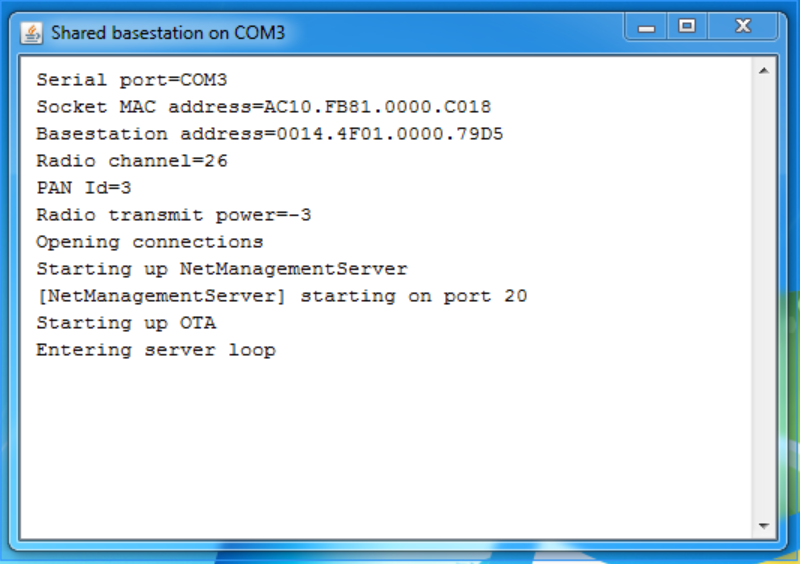
\includegraphics[scale=0.5]{Bilder/server}
	\caption{Logdaten der Basisstation bei Servererstellung}
	\label{f:server}
\end{figure}

Der zweite Teil der ‚run()‘-Methode besteht aus einer while-Schleife, welches auf ankommende Pakete wartet und diese entgegennimmt. Nur wenn der SPOT eine Bewegung erfährt, sendet er ein Paket an die Basisstation. So kann die Desktop-Applikation sicher sein, dass immer, wenn ein Paket gesendet wird, eine Bewegung stattfand.\\

\begin{lstlisting}[language=Java,caption={Auswerten des empfangenen Paketes},label=lst:rcvpackage,frame=single] 
while (true) {
	try {
		// Empfangen und Lesen des Pakets
		rCon.receive(dg);
		long time = dg.readLong();
		System.out.println(time);
		status.append("Bewegung festgestellt!\n");
		} 
	catch (Exception e) {
		System.err.println("Exception " + e +  " beim Lesen der Daten.");
		throw e;
		}
	}
\end{lstlisting}

Innerhalb des übermittelten Paketes befindet sich die aktuelle Uhrzeit, um die Bewegung nachher genau zeitlich einordnen zu können. Sobald die Desktop-Applikation ein Paket empfängt, gibt sie auf dem Bildschirm innerhalb des erstellten Frames den Text 'Bewegung festgestellt!' aus. So wird dem Nutzer unmissverständlich klar gemacht, dass der Sensor in Bewegung war.

\begin{figure}[H] 
	\centering
	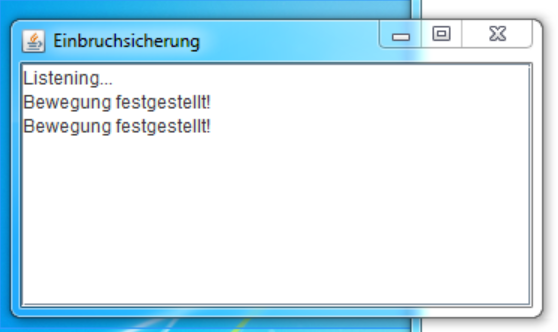
\includegraphics[scale=0.8]{Bilder/bewegung}
	\caption{JFrame mit textueller Ausgabe}
	\label{f:bewegung}
\end{figure}

Innerhalb der Konsole werden neben Debugausgaben zur Basisstation und die Liste eröffneter Ports der Zeitstempel, welcher mit der Bewegung vom SunSPOT übermittelt wird, ausgegeben.

\begin{figure}[H] 
	\centering
	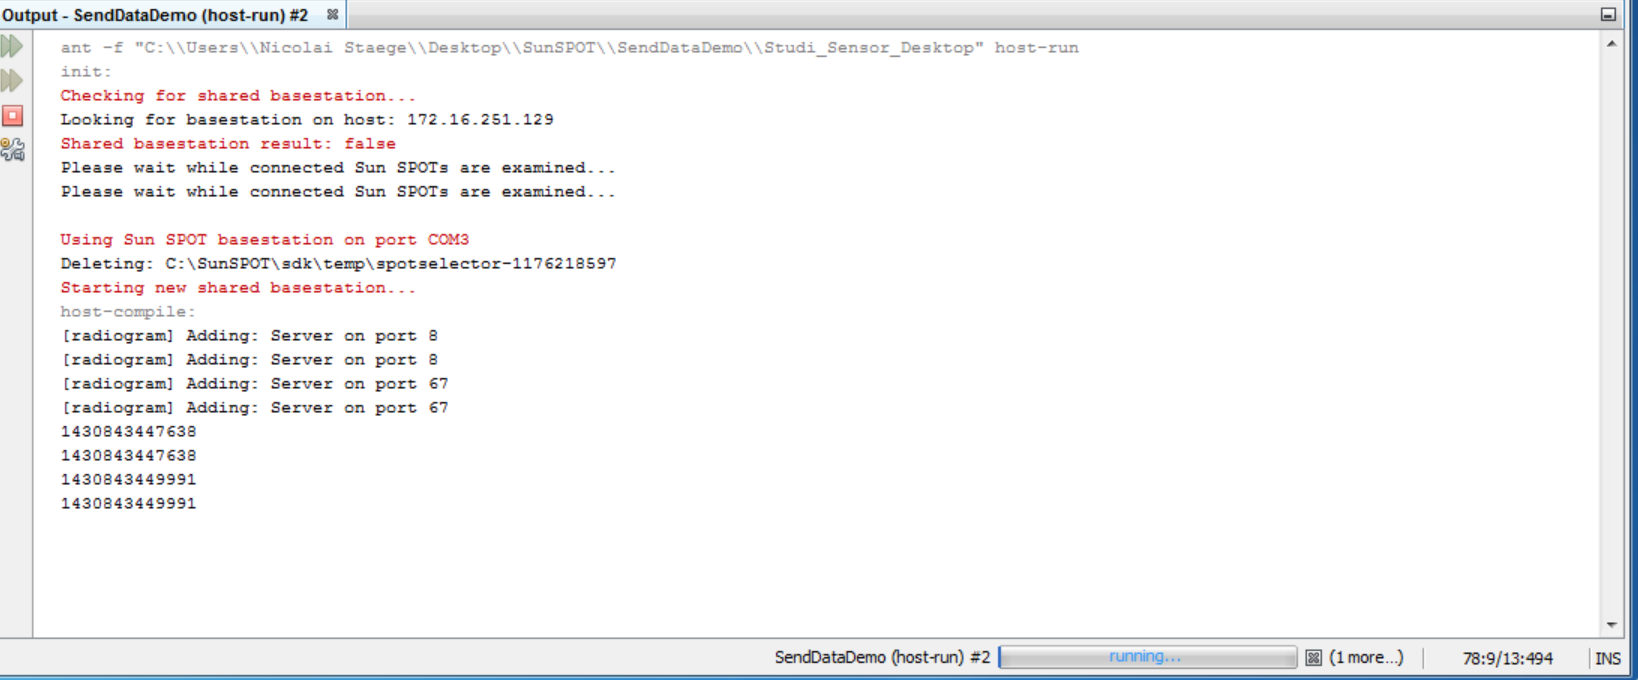
\includegraphics[scale=0.5]{Bilder/timestamp}
	\caption{Konsolenausgabe mit Timestamp}
	\label{f:timestamp}
\end{figure}

\subsubsection{SPOT-Applikation}\label{sss:SPOT-Applikation}